\FloatBarrier
\subsection{Question 7}
\autoref{code:str71}  is the necessary changes in the codebase to implement white and colored noise and related fixes in Indirect STR controller.  Effect of white noise on the system is shown in \autoref{fig:str71}.  \autoref{fig:str72} represents the variation on estimation parameters when white noise is present. By varying the $lamda$ of RLS, we can compensate for white noise as shown in  \autoref{fig:str73}.  \autoref{fig:str74} and  \autoref{fig:str75} present the output and parameter changes of the system when colored noise is applied to the output.  \autoref{fig:str76} presents the fixed output of the system with colored noise. By varying the $R$ parameter and $Lamda$ and introducing further $A_o$ polynomial roots we can compensate for colored noise.

\begin{code}
	\begin{matlabcode}{firstnumber = 1}
noise = 1; % if 1 white noise, 2 colored noise
lamda = 0.9;
. . .
if noise
	e = 0.05*randn(length(t),1);
	if noise == 2
		sys_dist = tf(1,[1 -1] , Gz.Ts) ;
		ynoise = lsim(sys_dist , e , t) ;
	else
		ynoise = e;
	end
else
	ynoise = zeros(length(t),1);
end
. . .
    y(i) = -A(2:end)*y(i-1:-1:i-na)+B*(u(i-d0:-1:i-na)+vdist(i-(numel(A)-numel(B)):-1:i-(numel(A)-1))+ynoise(i-(numel(A)-numel(B)):-1:i-(numel(A)-1))) ;

	\end{matlabcode}
	\captionof{listing}{Noise implementation in Indirect STR}
	\label{code:str71}
\end{code}

\begin{figure}
	\centering
	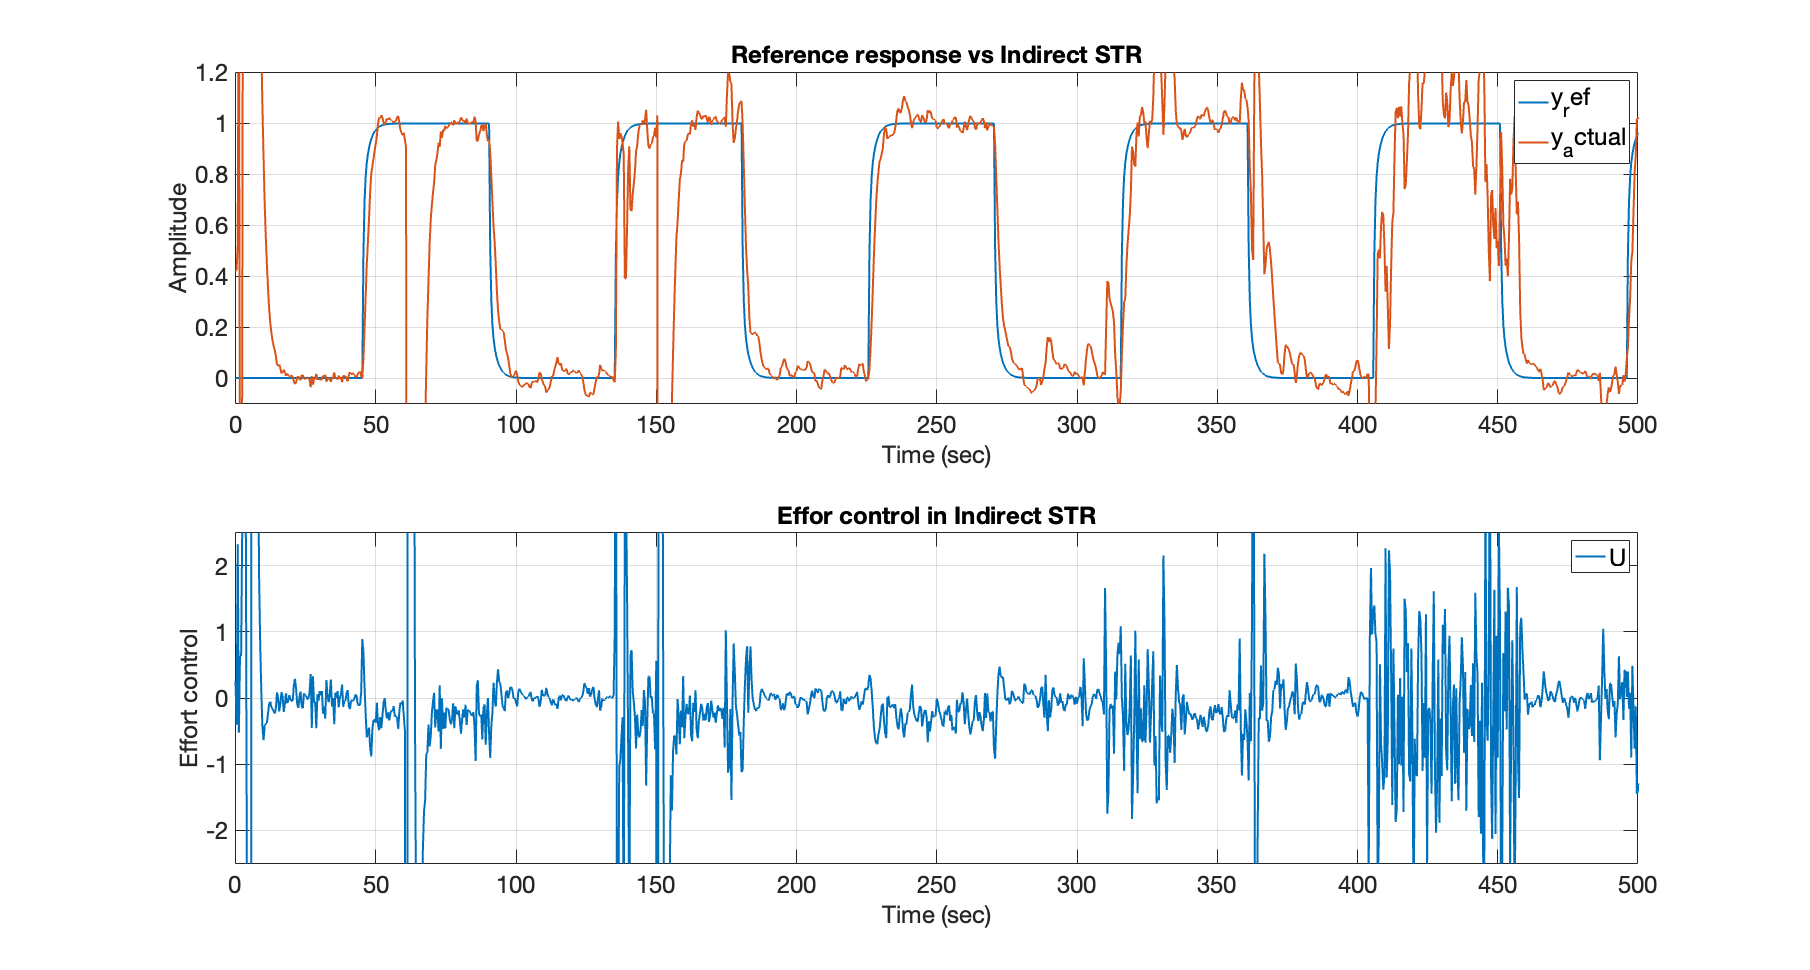
\includegraphics[width=\textwidth]{images/str71.png}
	\caption{System output with white noise}
	\label{fig:str71}
\end{figure}

\begin{figure}
	\centering
	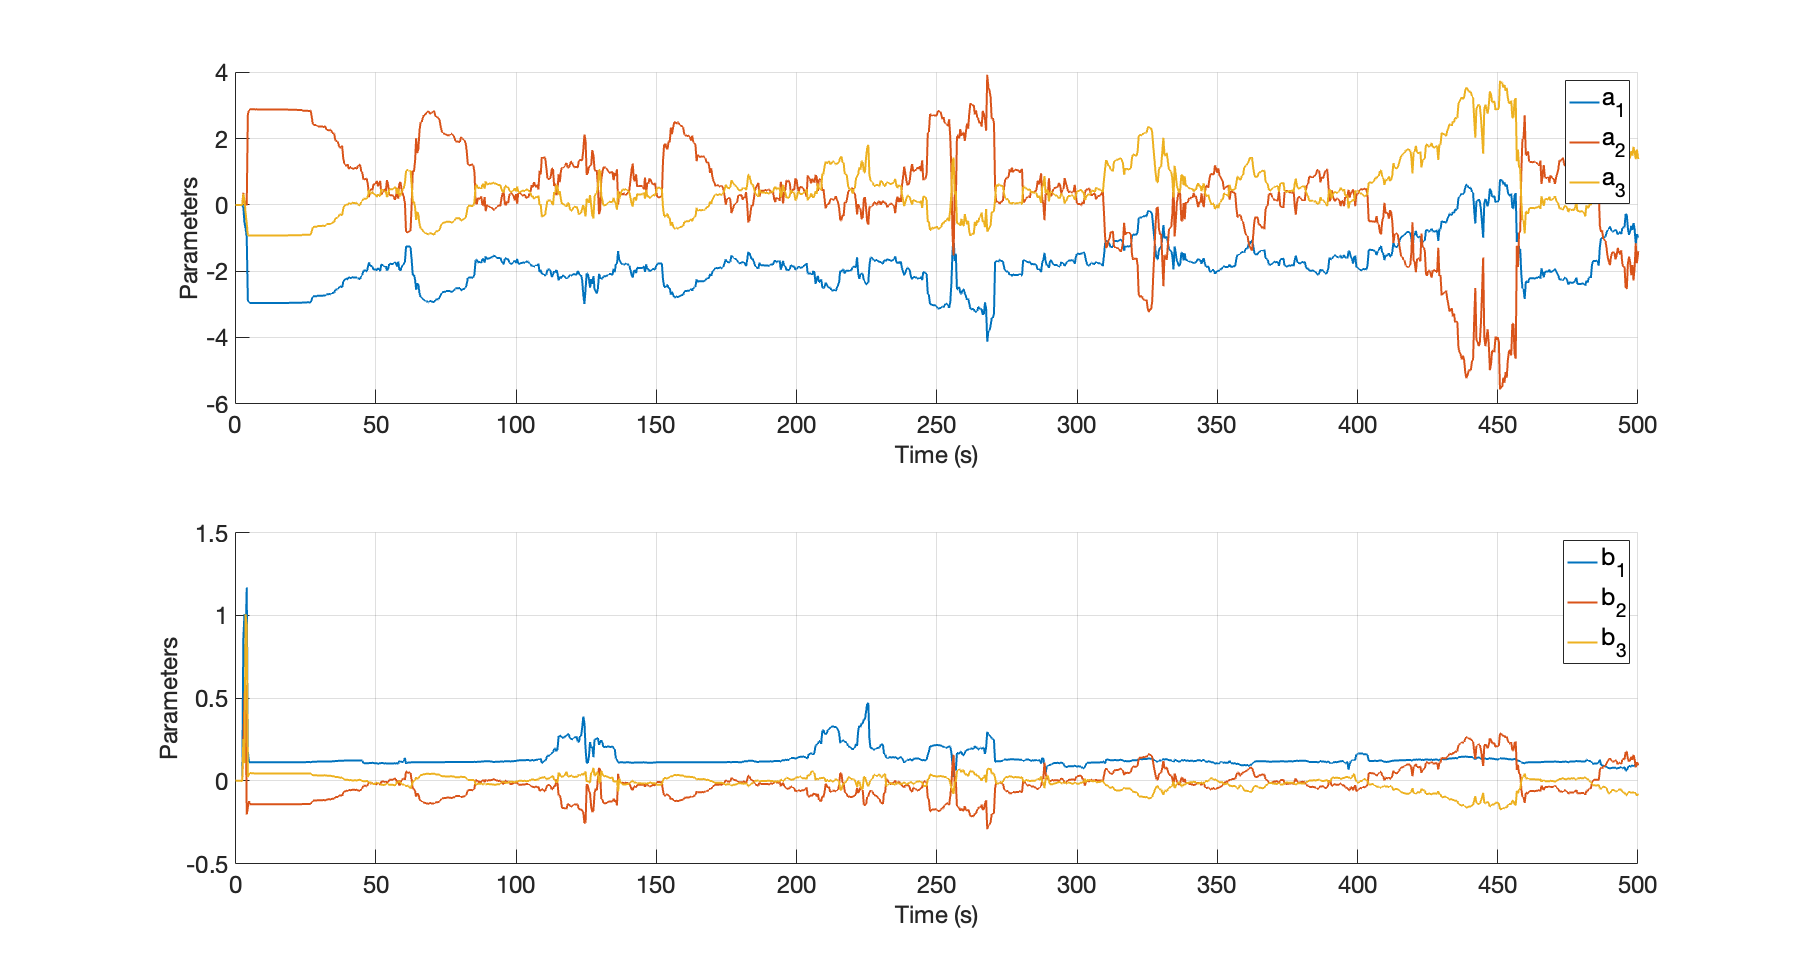
\includegraphics[width=\textwidth]{images/str72.png}
	\caption{System parameters with white noise}
	\label{fig:str72}
\end{figure}

\begin{figure}
	\centering
	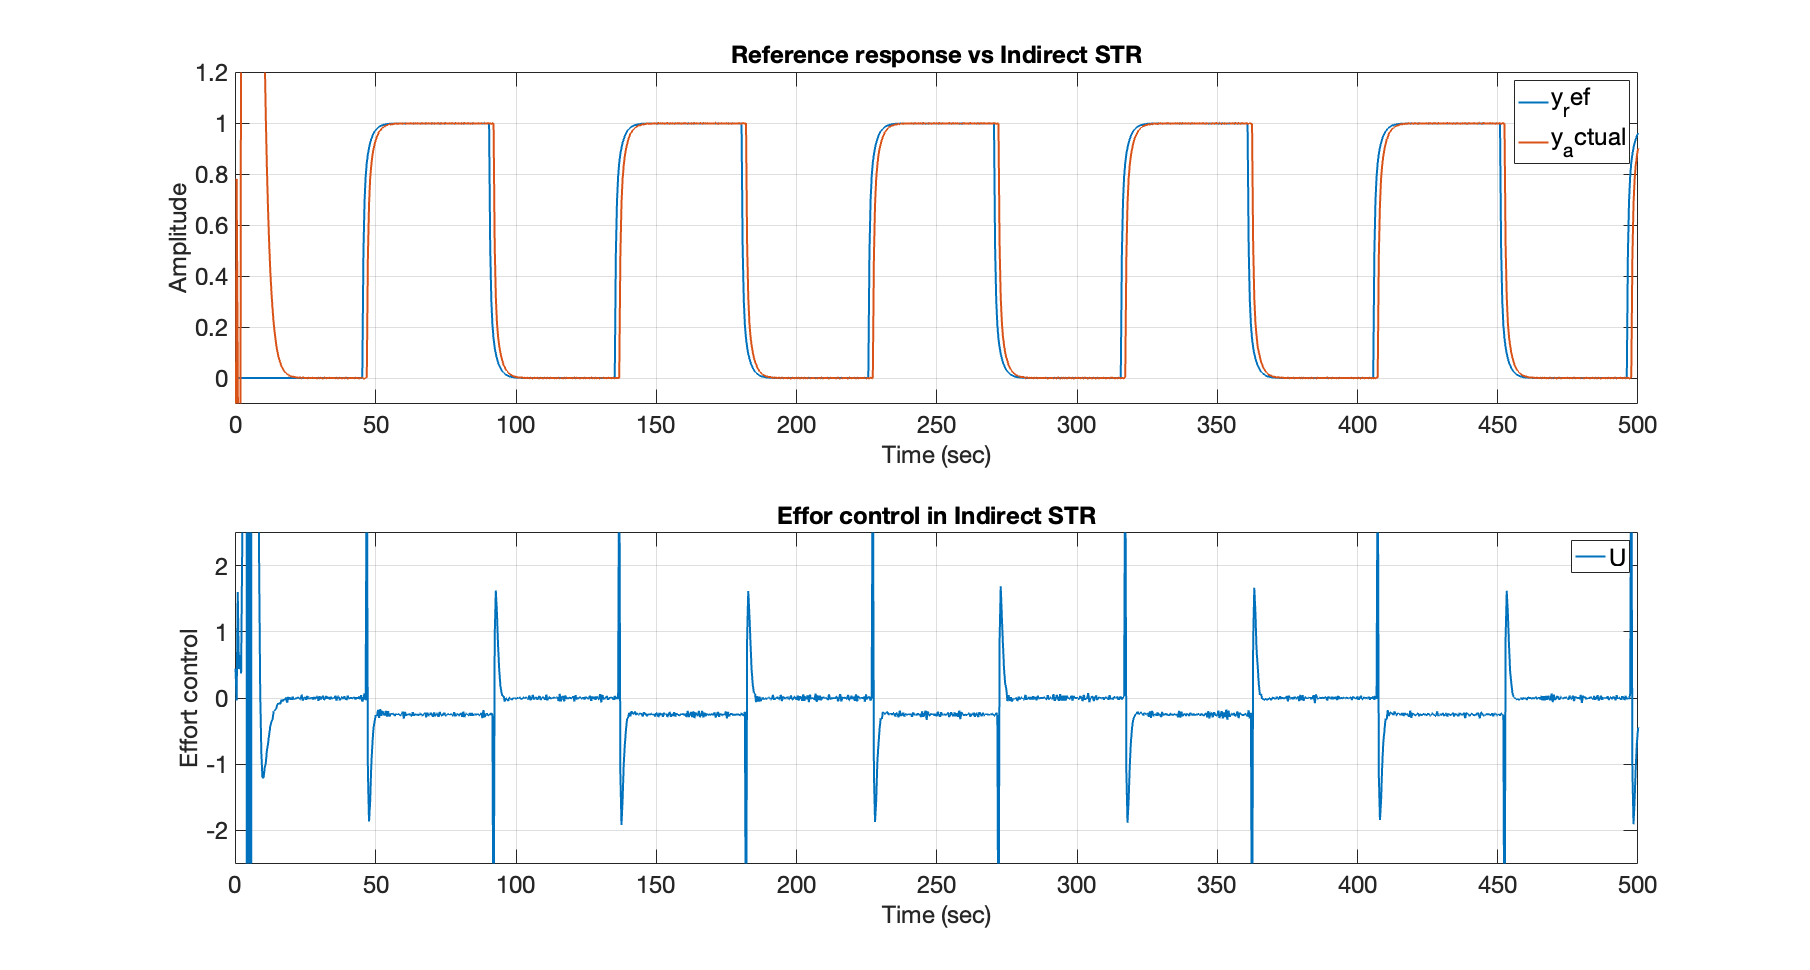
\includegraphics[width=\textwidth]{images/str73.png}
	\caption{Compensating for system with white nois}
	\label{fig:str73}
\end{figure}

\begin{figure}
	\centering
	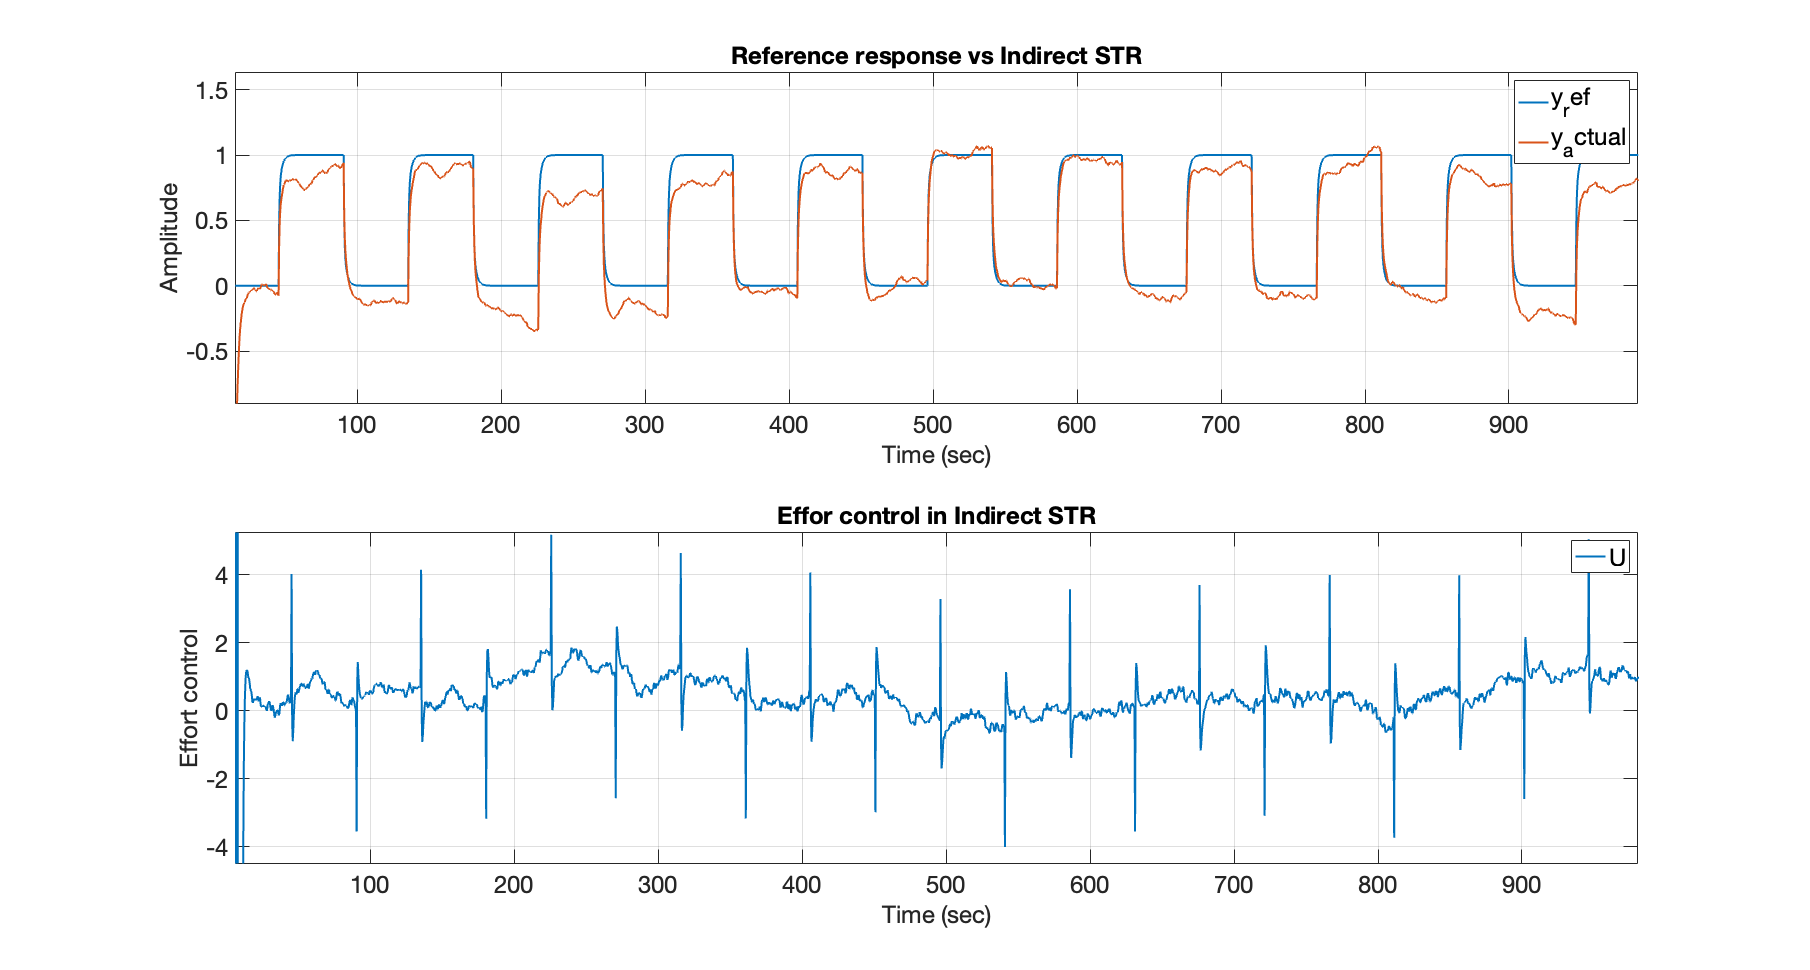
\includegraphics[width=\textwidth]{images/str74.png}
	\caption{System output with colored noise}
	\label{fig:str74}
\end{figure}

\begin{figure}
	\centering
	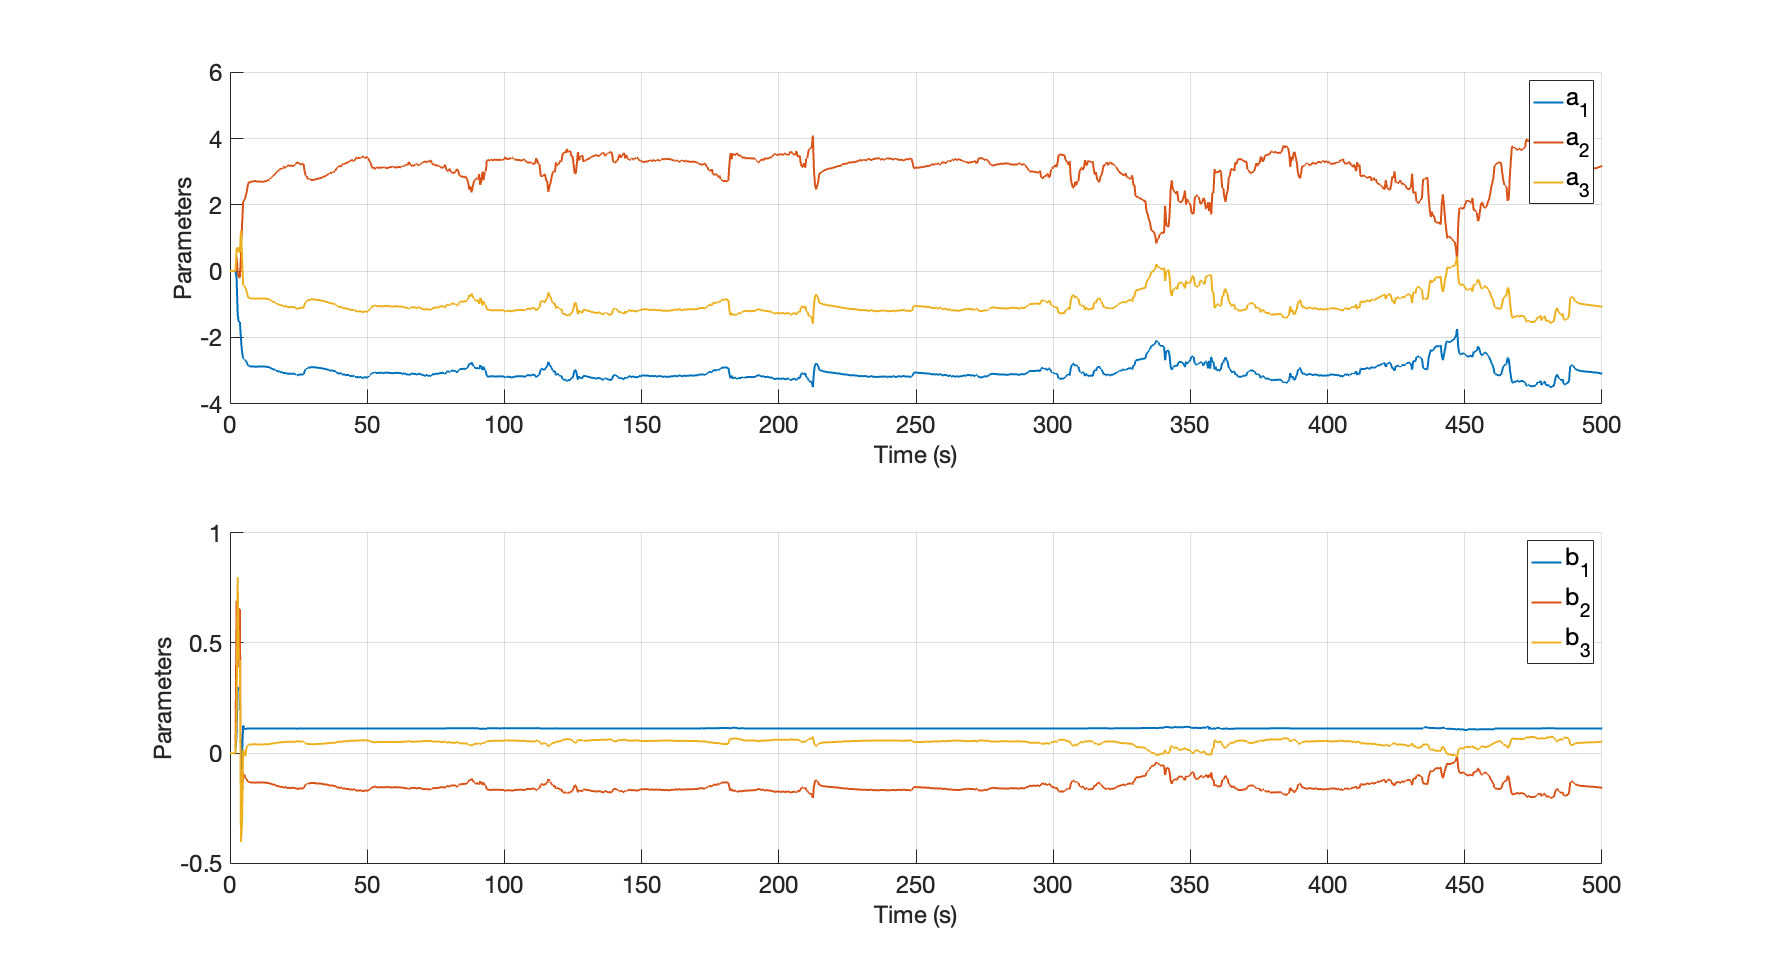
\includegraphics[width=\textwidth]{images/str75.png}
	\caption{System parameters with colored noise }
	\label{fig:str75}
\end{figure}

\begin{figure}
	\centering
	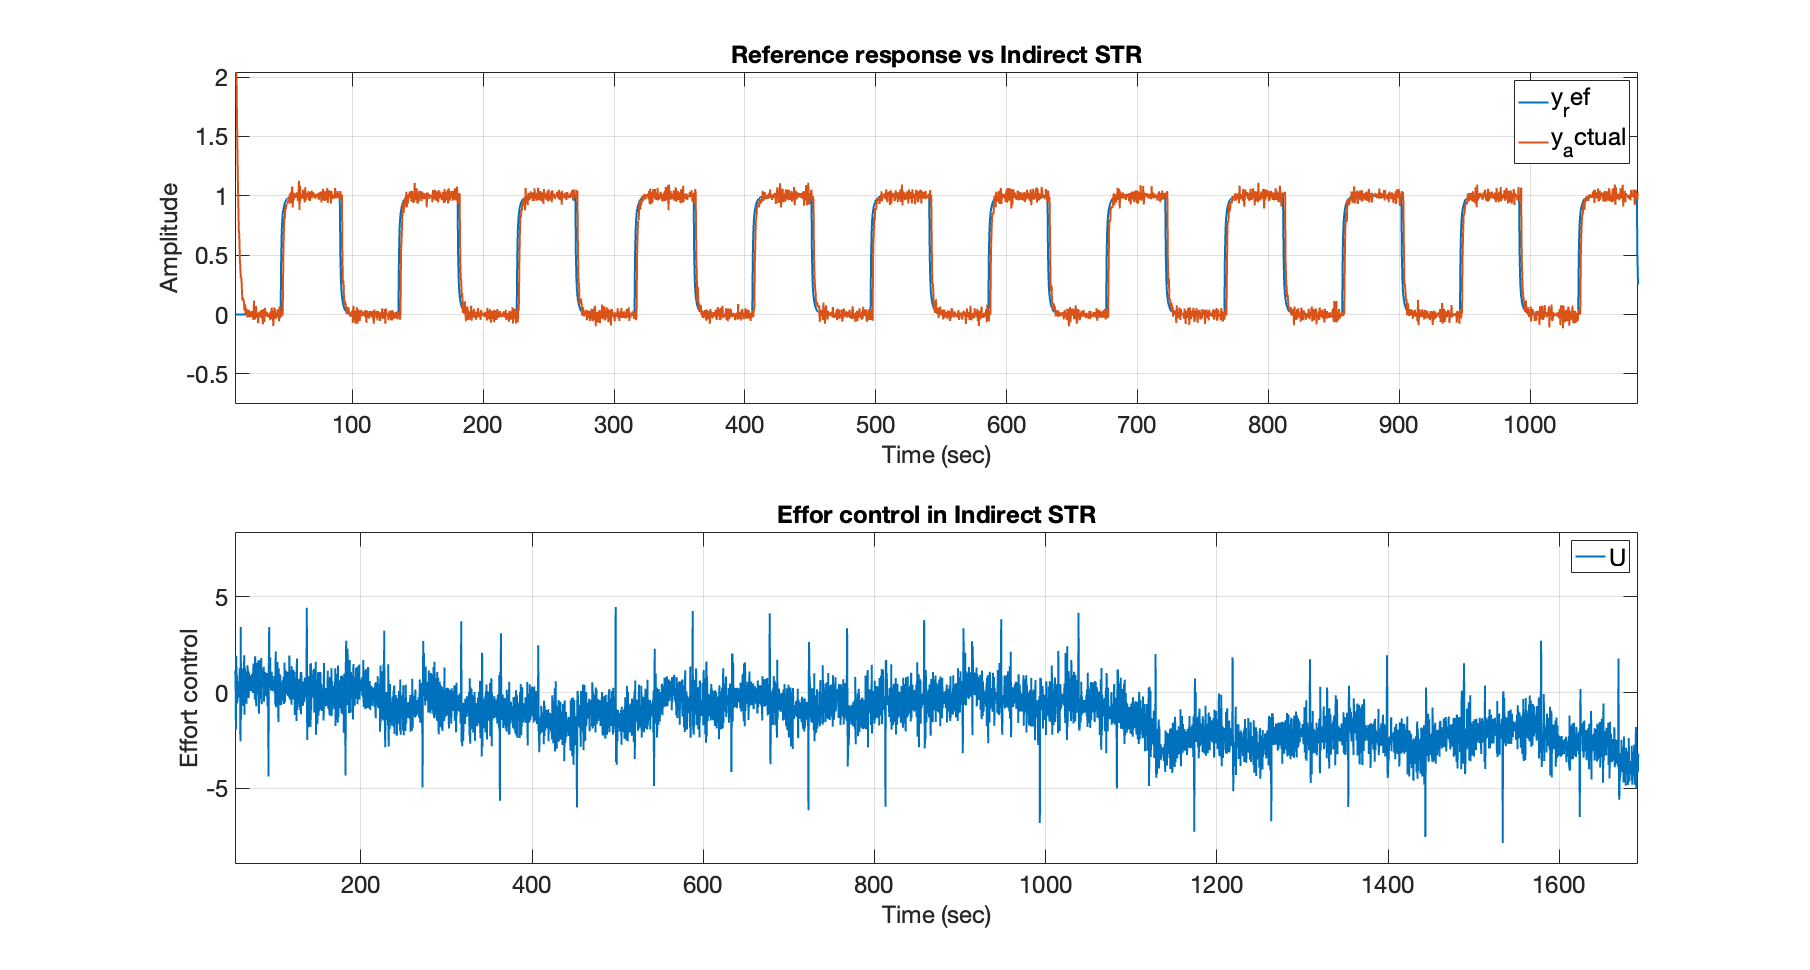
\includegraphics[width=\textwidth]{images/str76.png}
	\caption{Compensating for system with colored noise }
	\label{fig:str76}
\end{figure}
The code  for this section is available at \lstinline|assignment2/part2/STR1_indirect.m|. By changing the $noise=0$ to $1$ we can introduce white noise to the system. changing the same variable to $2$ implements a colored noise in the system. $lamda$ is used as a forgetting factor for RLS.
